
\chapter{Demonstration}
%%%%%%%%%%
\label{chap:demo}

\acrshort{DSR} demands a use of the artifact in at least one use case. In case of reference modeling, the model's purpose in practice is its application, which is its demonstration. 

Arvato, introduced in chapter \ref{chap:case}, is subject to the instantiation of the domain reference model to a provider model (\cf \Fig \ref{fig:modellevels}). The provider model intentionally embodies individual characteristics, so that changes to the domain reference model are inevitable. These changes specialize, but do not contradict research in this thesis. 

Documents and interview transcripts are foundation of the following practical exhibition. 



	\section{Process Framework}
	
	Starting point is the most abstract level of the model, \ie the framework.
	 \Tab \ref{tab:interv} gives an overview about covered aspects in interviews. The interviews cover all processes, except \textsc{Inbound Service} and \textsc{Outbound Service}. For these, results from the process modeling workshop are available. The author was part of the workshop and conducted all interviews. 

\begin{table}[caption={Interviews and Relations to Processes}, label={tab:interv}]
	\centering
	
	\begin{tabular}{p{1cm} p{3.4cm}  p{4cm}  p{5cm} }
		\textbf{Order} & \textbf{Topic} & \textbf{Interviewee}          & \textbf{Relation to Processes}                          \\ \hline \hline
		1                            & Model expectations            & Member of the board                  &                                                                         \\\hline
		2                            & Sales                         & Global sales manager                 & \textsc{Sales}, \textsc{Transition}                                                       \\\hline
		3                            & IT                            & Global IT manager                    & \textsc{Transition}                                                              \\\hline
		4                            & Operations                    & Global operations manager            & \textsc{Quality}, \textsc{People Lifecycle}, \textsc{Operations Management} \\\hline
		5                            & Portfolio \& Solution Design  & Global portfolio manager             & \textsc{Product Development}, \textsc{Portfolio Management}, \textsc{Solution Design }             \\\hline
		6                            & Solution Design \& Consulting & Senior consultant                    & \textsc{Product Development}, \textsc{Portfolio Management}, \textsc{Solution Design}              \\\hline
		7                            & Self-Service technologies     & Global portfolio \& solution manager & \textsc{Self-Services}, \textsc{Solution Design}, \textsc{Knowledge Management}                     \\\hline
		8                            & Account Management            & Key account manager                  & \textsc{Transition}, \textsc{Account Management  }                                                    \\\hline
		9                            & Implementation                & Global sales manager                 & \textsc{Transition}                                                             
	\end{tabular}
\end{table}

	Regarding the overall split into management, client and customer processes, interviewees conveyed that Arvato divides into global and local responsibilities. These are on the one hand subject to country organizations, but on the other hand relate to specific client businesses. The five managerial processes have their global pendant at Arvato, included in the research through interview partner with a global range of activity. The split regarding client and customer processes is seen in the organization's units \textit{Sales \& Business Development} and \textit{Operations}, respectively (\cf \ref{chap:case:org}). The provider model is shown in \Fig \ref{fig:arvatofram} and discussed below.
	
\begin{figure}[caption={Arvato Framework}, label={fig:arvatofram}]
	{	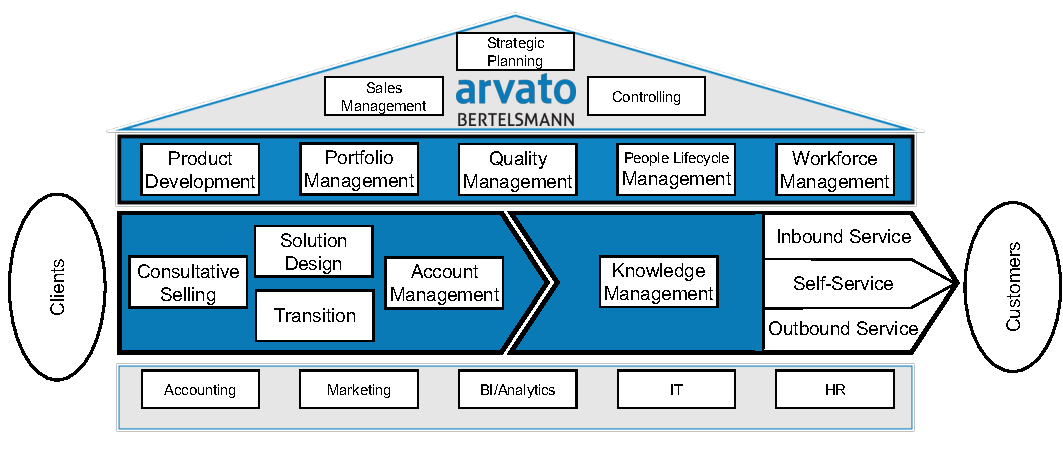
\includegraphics[width=.98\textwidth]{figures/frameworkA.pdf} 
	}
\end{figure}


	%%%%%%%%%%
	%%%%%%%%%%
	
	\section{Customer Processes}
	
	Practical evidence for the four processes in this area is seen in the interview regarding self-services (relating to \textsc{Self-Services} and \textsc{Knowledge Management}) and the process modeling workshop (relating to \textsc{Inbound} and \textsc{Outbound Services}). 
		\subsection{Inbound \& Outbound Services}
	Building on the workshop at one location covering multiple clients in tourism and financial services, a clear picture about operations in a contact center was captured. 
	As voice, video, email, chat, twitter and facebook interactions were covered, all four channel types introduced in this thesis (voice, mail, direct messenger, social) have been explored. As participating managers shared their perception on inter-personal service interactions across client businesses located at their site, an abstraction from client-specific details can be assumed. The outcomes of the workshop were generalized to approximate the detail level within the process reference model. \textsc{Inbound Service} and \textsc{Outbound Service}, as modeled in \ref{pr:inb}, \ref{pr:out}, cover more aspects than found in the workshop outcomes. As analytical support was very limited and no central customer database was existing, several reference model process steps have to be seen as optional in an application on this client case. However, as one specific client business is seen as a client model instead of a provider model, the supported optionality of process steps in icebricks protects integrity. An omission of these optional steps in the client model can be realized.
	
	\subsection{Self-Services \& Knowledge Management}
	The interviewee saw customer needs in center of \textsc{Self-Service}, which is aligned to the reference process. However, it was admitted that difficulties arise in a process representation, because the diversity of self-service utilization implies different procedures. The representation in this work corresponds to the \textit{maintenance} phase of self-service technologies, which follows the \textit{project} phase according to the interviewee. The latter describes the implementation of a self-service and can be seen as part of client processes in the reference model. However, the maintenance phase especially consists of back-end processes, that are covered in \textsc{Knowledge Management}. Explicitly the creation and maintenance of content \wrt customer needs was mentioned in this regard. The proposed case-, transaction-, and customer-related knowledge split in the reference process is hence supported regarding the \textit{case} dimension. However, customer- and transaction-related knowledge was deemed important in inter-personal services and therefore \textsc{Knowledge Management} is seen as applicable to Arvato. 
	
	\textsc{Self-Service} is modeled from a system perspective, therefore it must adequately represent used self-service systems from Arvato. Chat bots and semantic search can be named to give a channel-integrated and stand-alone example. While a chat bot must perform the reference process for every message in a conversion, a single passing through the steps can represent a semantic search. The abstract \textit{customer need}  object enables the demonstration of both applications in the reference process.   

	Regarding terminology, the notion \textit{next best action} shall be used instead of \textit{resolution}. 
	%%%%%%%%%%
	%%%%%%%%%%
	\section{Client Processes}
	By ordering the interviews regarding their relation to the outsourcing lifecycle, interview 2,3,9 and 8 can be named. \textsc{Solution Design} is subject of interview 5,6 and 7 of \Tab \ref{tab:interv}.
	
	While the general structure of the framework is seen as applicable to Arvato, a customization is applied to emphasize strategic priorities of the organization for its provider model. \textsc{Sales} is renamed \textsc{Consultative Selling}, as it was seen as differentiating Arvato from competitors. 
	
	\subsection{Consultative Selling}
	
	This approach puts more emphasis on proactive activities in pre-sales, which is seen in the first two detail processes of \textsc{Sales} (\textit{identify prospect} and \textit{approach prospect}). The following steps conform to \textit{Bid Management} at Arvato, where a detailed process description is existing that matches the reference detail processes. For the provider model, this documentation is used to specify process building blocks (\cf Appendix \ref{app:salesbb}). 	The importance of \acrshort{RFP} is stressed by Arvato, which is conforming to the reference model. \textit{Perform due diligence} \textit{negotiate contract} and \textit{create commercial deal} are not explicitly listed as parallel processes, but covered in the documentation. Contract creation is seen as part of \textit{Contract Management} at Arvato. 
	
	\subsection{Transition}
	
	Implementation or transition are used to describe the phase between a signed contract and start of final operational service delivery. As discussed in \ref{pr:tra}, it was affirmed that the process starts during contract finalization, which also supports a separate modeling on framework level. Due diligence was seen as an important supporting factor to plan with less uncertainty. A transition plan was not explicitly mentioned, but it can be assumed that information is compiled in one or more documents that structure the transition project. 
	
	The interviewee stated that the most important question in this process is about the location of knowledge and documentation, which is captured in the \textit{transfer business, people, process, technology} detail processes. The proposal to segment into people, process and technology was consented. In addition, the initial recruiting and training of \acrshort{CSR}s was named, which is found under \textsc{People Lifecycle Management} in the reference model. 
	
	While \acrshort{PMO} and \acrshort{TMO} phase were not found explicitly mentioned, their concepts were expressed during the interview. It was stated that it is recommended to start the transfer without further changes (corresponding \acrshort{PMO}). After this phase, optimization of status-quo (\ie, \acrshort{TMO}) can be initiated. 
	
	\subsection{Account Management}
	 \textsc{Sales} and \textsc{Account Management} can be linked together in country organizations inside Arvato. This view was taken in interview 8 and therefore a scoping of process boundaries was necessary. The starting point of the \textsc{Account Management} was seen at the latest with signing of the contract and therefore exists during \textsc{Transition}. Constituents of the reference process were named in the interview, namely service performance monitoring, contract management and especially relationship management. Change management is not explicitly modeled as a detail process, but captured in \textit{manage disputes} \textit{propose innovation} and \textit{renegotiate contract}. As a lifecycle analogy was stated, \textit{end contract} is a suitable last detail process. 
          
   	\subsection{Solution Design}
	\textsc{Solution Design} as a process in the reference model corresponds to a same-named organizational unit within Arvato. 

	\section{Management Processes}
	%%%%%%%%%%
	\subsection{Product Development}
	SD: plattform noch nicht definiert
	
	\subsection{Portfolio Management}
	sales und delivery portfolio
	communication wird in SD genannt
	
	
	\subsection{Quality Management}
	\subsection{People Lifecycle Management}
	\subsection{Operations Management}
	
